% Generated by tex/build_swebok_structure.py from tex/chapters/ch01/08_要求管理活動.tex
\subsubsection{範囲調整}

\term{範囲調整}とは、作るべき要求の範囲が、費用、納期、人員などの制約を超えないように調整する活動である。範囲が大きすぎる場合には、要求を減らす、予算や人員を増やす、納期を延ばす、またはそれらを組み合わせる必要がある。

可能であれば、範囲調整は感覚ではなく、機能規模、工数、リスクなどの測定値に基づいて行うとよい。

\begin{figure}[htbp]
\centering
\IfFileExists{swebok_structure/CH01.ソフトウェア要求(Software_Requirements)/1.6.要求管理活動(Requirements_Management_Activities)/1.6.3.範囲調整(Scope_Matching)/assets/fig-ch01-10.png}{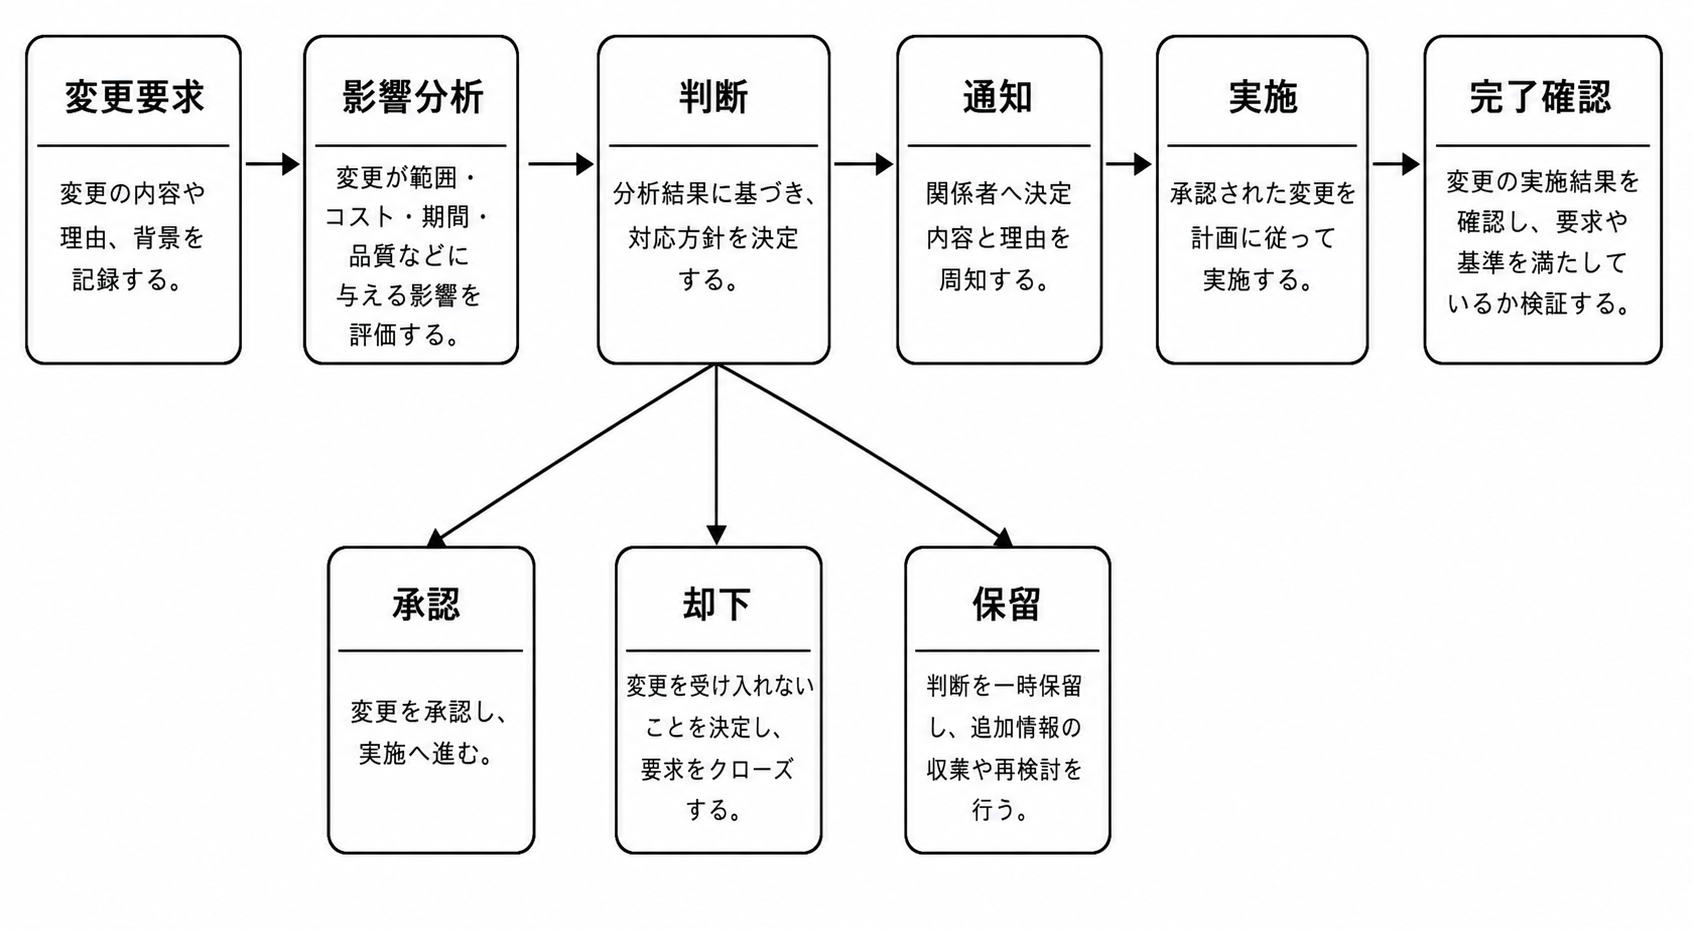
\includegraphics[width=0.96\linewidth]{swebok_structure/CH01.ソフトウェア要求(Software_Requirements)/1.6.要求管理活動(Requirements_Management_Activities)/1.6.3.範囲調整(Scope_Matching)/assets/fig-ch01-10.png}}{\fbox{\parbox[c][48mm][c]{0.9\linewidth}{\centering 画像生成待ち\\要求変更管理の流れ}}}
\caption{要求変更管理の流れ}
\label{fig:ch01-10}
\end{figure}
